% Para utilizar este template siga o tutorial disponível em http://www.biblioteca.ufc.br/wp-content/uploads/2015/09/tutorial-sharelatex.pdf

%%%%%%%%%%%%%%%%%%%%%%%%%%%%%%%%%%%%%%%%%%%%%%%%%%%%%%%
%% Você deve criar uma conta no Overleaf. Depois,    %%
%% vá nas opções no canto esquerdo superior da tela  %%
%% e clique em "Copiar Projeto". Dê um novo nome pa- %%
%% ra o projeto.                                     %%
%%                                                   %%
%% Os principais desenvolvedores deste template são: %%
%%                                                   %%
%%            Ednardo Moreira Rodrigues              %%
%%       (Doutor em Engenharia Elétrica - UFC)       %%
%%                      &                            %%
%%            Alan Batista de Oliveira               %%
%%           (Engenheiro Eletricista - UFC)          %%
%%                                                   %%
%% Consultoria Bibliotecária                         %%
%%                                                   %%
%%  Versão 2016 - ShareLaTeX:                        %% 
%%                                                   %%
%% - Francisco Edvander Pires Santos;                %%
%% - Juliana Soares Lima;                            %%
%% - Izabel Lima dos Santos;                         %%
%% - Kalline Yasmin Soares Feitosa;                  %%
%% - Eliene Maria Vieira de Moura.                   %%
%%
%%  Versão 2019 - Overleaf:
%%  
%%  Biblioteca de Ciências Humanas: 
%% - Francisco Edvander Pires Santos;                %%
%% - Juliana Soares Lima;                            %%
%% - Eliene Maria Vieira de Moura;                   %%
%% - Edmundo Moreira de Sousa Filho.                 %%
%%                                                   %%
%% Biblioteca da FEAAC:                              %%
%% - Izabel Lima dos Santos;                         %%
%% - Kalline Yasmin Soares Feitosa;                  %%
%% - Kleber Lima dos Santos.                         %%
%%                                                   %%
%%  Biblioteca do Curso de Física:                   %%
%% - Aline Rodrigues de Lima Mendes;                 %%
%% - Maria de Jesus Silva dos Santos.                %%
%%                                                   %%
%%  Biblioteca Central do Campus do Pici:            %%
%% - Raquel da Silva Nascimento.                     %%
%%                                                   %%
%% Colaboradores                                     %%
%%                                                   %%
%% -Andrei Bosco Bezerra Torres                      %% 
%% (Professor - Sistemas e Mídias Digitais -         %%
%% Instituto Universidade Virtual - UFC)             %%
%% Tiago ALves Lima                                  %% 
%% (Aluno de Mestrado em Eng. Elétrica)              %%
%%                                                   %%
%% Grande parte do trabalho foi adaptado do template %%
%% da UECE elaborado por:                            %%
%% Thiago Nascimento  (UECE)                         %%
%% Project available on:                             %%
%% https://github.com/thiagodnf/uecetex2             %%
%%                                                   %%
%% "Dúvidas, esclarecimentos ou sugestões podem ser  %%
%% enviadas para o seguinte e-mail:                  %%
%%                                                   %%
%%             atendimentobch@ufc.br                 %%
%%                                                   %%
%% As últimas atualizações estão descritas no inicio %%
%% do arquivo "README.md".                           %%
%%                                                   %%
%%%%%%%%%%%%%%%%%%%%%%%%%%%%%%%%%%%%%%%%%%%%%%%%%%%%%%%

\documentclass[        
    a4paper,          % Tamanho da folha A4
    12pt,             % Tamanho da fonte 12pt
    chapter=TITLE,    % Todos os capitulos devem ter caixa alta
    section=Title,    % Todas as secoes devem ter caixa alta somente na primeira letra
    subsection=Title, % Todas as subsecoes devem ter caixa alta somente na primeira letra
    oneside,          % Usada para impressao em apenas uma face do papel
    english,          % Hifenizacoes em ingles
    spanish,          % Hifenizacoes em espanhol
    brazil,           % Ultimo idioma eh o idioma padrao do documento
    fleqn             % Comente esta linha se quiser centralizar as equacoes. Comente também a linha 65 abaixo
]{abntex2}

% Para utilizar este template siga o tutorial disponível em http://www.biblioteca.ufc.br/wp-content/uploads/2015/09/tutorial-sharelatex.pdf

%%%%%%%%%%%%%%%%%%%%%%%%%%%%%%%%%%%%%%%%%%%%%%%%%%%%%%%
%% Você deve criar uma conta no Overleaf. Depois,    %%
%% vá nas opções no canto esquerdo superior da tela  %%
%% e clique em "Copiar Projeto". Dê um novo nome pa- %%
%% ra o projeto.                                     %%
%%                                                   %%
%% Os principais desenvolvedores deste template são: %%
%%                                                   %%
%%            Ednardo Moreira Rodrigues              %%
%%       (Doutor em Engenharia Elétrica - UFC)       %%
%%                      &                            %%
%%            Alan Batista de Oliveira               %%
%%           (Engenheiro Eletricista - UFC)          %%
%%                                                   %%
%% Revisão:                                          %%
%%                                                   %%
%% - Francisco Edvander Pires Santos;                %%
%% - Juliana Soares Lima;                            %%
%% - Izabel Lima dos Santos;                         %%
%% - Kalline Yasmin Soares Feitosa.                  %%
%% - Eliene Maria Vieira de Moura;                   %%
%%                                                   %%
%% Colaboradores                                     %%
%%                                                   %%
%% -Andrei Bosco Bezerra Torres                      %% 
%% (Professor - Sistemas e Mídias Digitais -         %%
%% Instituto Universidade Virtual - UFC)             %%
%% Tiago ALves Lima                                  %% 
%% (Aluno de Mestrado em Eng. Elétrica)              %%
%%                                                   %%
%% Grande parte do trabalho foi adaptado do template %%
%% da UECE elaborado por:                            %%
%% Thiago Nascimento  (UECE)                         %%
%% Project available on:                             %%
%% https://github.com/thiagodnf/uecetex2             %%
%%                                                   %%
%% "Dúvidas, esclarecimentos ou sugestões podem ser  %%
%% enviadas para o seguinte e-mail:                  %%
%%                                                   %%
%%             atendimentobch@ufc.br                 %%
%%                                                   %%
%% As últimas atualizações estão descritas no inicio %%
%% do arquivo "README.md".                           %%
%%                                                   %%
%%%%%%%%%%%%%%%%%%%%%%%%%%%%%%%%%%%%%%%%%%%%%%%%%%%%%%%

% Importações de pacotes
\usepackage[utf8]{inputenc}                         % Acentuação direta
\usepackage[T1]{fontenc}                            % Codificação da fonte em 8 bits
\usepackage{graphicx}                               % Inserir figuras
\usepackage{amsfonts, amssymb, amsmath}             % Fonte e símbolos matemáticos
\usepackage{booktabs}                               % Comandos para tabelas
\usepackage{verbatim}                               % Texto é interpretado como escrito no documento
\usepackage{multirow, array}                        % Múltiplas linhas e colunas em tabelas
\usepackage{indentfirst}                            % Endenta o primeiro parágrafo de cada seção.
\usepackage{listings}                               % Utilizar codigo fonte no documento
\usepackage{xcolor}
\usepackage{microtype}                              % Para melhorias de justificação?
\usepackage[portuguese,ruled,lined]{algorithm2e}    % Escrever algoritmos
\usepackage{algorithmic}                            % Criar Algoritmos  
%\usepackage{float}                                 % Utilizado para criação de floats
\usepackage{amsgen}
\usepackage{lipsum}                                 % Usar a simulação de texto Lorem Ipsum
%\usepackage{titlesec}                              % Permite alterar os títulos do documento
\usepackage{tocloft}                                % Permite alterar a formatação do Sumário
\usepackage{etoolbox}                               % Usado para alterar a fonte da Section no Sumário
\usepackage[nogroupskip,nonumberlist]{glossaries}   % Permite fazer o glossario

\usepackage[font=singlespacing,format=plain,justification=justified,skip=0pt,singlelinecheck = false]{caption}            % Altera o comportamento da tag caption

\usepackage[alf, abnt-emphasize=bf, recuo=0cm, abnt-etal-cite=2, abnt-etal-list=0, abnt-etal-text=it]{abntex2cite}  % Citações padrão ABNT
%\usepackage[bottom]{footmisc}                      % Mantém as notas de rodapé sempre na mesma posição
%\usepackage{times}                                 % Usa a fonte Times
%%%%%%%%%%%%%%%%%%% AVISO %%%%%%%%%%%%%%%%%%%%%%%%%%%%%%%%%%%%%%%%
%descomente as duas linhas abaixo para alterar o texto de Times New Roman para Arial:

%\usepackage{helvet}
%\renewcommand{\familydefault}{\sfdefault}  % Usa a fonte Arial              
%%%%%%%%%%%%%%%%%%%%%%%%%%%%%%%%%%%%%%%%%%%%%%%%%%%%%%%%%%%%%%%%%%

\usepackage{mathptmx}         % Usa a fonte Times New Roman			%\usepackage{lmodern}         % Usa a fonte Latin Modern
%\usepackage{subfig}          % Posicionamento de figuras
%\usepackage{scalefnt}        % Permite redimensionar tamanho da fonte
%\usepackage{color, colortbl} % Comandos de cores
%\usepackage{lscape}          % Permite páginas em modo "paisagem"
%\usepackage{ae, aecompl}     % Fontes de alta qualidade
%\usepackage{picinpar}        % Dispor imagens em parágrafos
%\usepackage{latexsym}        % Símbolos matemáticos
%\usepackage{upgreek}         % Fonte letras gregas
\usepackage{appendix}         % Gerar o apendice no final do documento
\usepackage{paracol}          % Criar paragrafos sem identacao
\usepackage{lib/ufctex}	      % Biblioteca com as normas da UFC para trabalhos academicos
\usepackage{pdfpages}         % Incluir pdf no documento
\usepackage{amsmath}          % Usar equacoes matematicas

\makeglossaries % Organiza e gera a lista de abreviaturas, simbolos e glossario
\makeindex      % Gera o Indice do documento

% --- Macros específicas do TCC (harness arquitetural) ------------------------
\usepackage{tabularx}                               % tabelas com largura total (\textwidth)
\usepackage{siunitx}                                % unidades: \SI{12.4}{\joule}, \si{\joule\per\token}
\sisetup{locale = DE, output-decimal-marker = {,}}

% Marcador de pendência no texto — some do PDF final ao trocar \newcommand por
% \newcommand{\pendencia}[1]{}
\newcommand{\pendencia}[1]{\textcolor{red}{[PENDENTE: #1]}}

% Termos recorrentes — mudar aqui muda o documento inteiro
\newcommand{\harness}{\textit{harness}}
\newcommand{\versaoH}{versão~H}
\newcommand{\versaoD}{versão~D}




\setlength{\mathindent}{0pt} %Complementa o alinhamento de equações para totalmente a esquerda.

%%%%%%%%%%%%%%%%%%%%%%%%%%%%%%%%%%%%%%%%%%%%%%%%%%%%%
%%                     ATENCAO                     %%
%%%%%%%%%%%%%%%%%%%%%%%%%%%%%%%%%%%%%%%%%%%%%%%%%%%%%
%  Qual e o nivel do trabalho academico que voce esta 
% escrevendo? Retire o simbolo "%" apenas de um dos 
% quatro topicos abaixo refente ao nível do seu traba
% -lho.

\trabalhoacademico{tccgraduacao}
%\trabalhoacademico{tccespecializacao}
%\trabalhoacademico{dissertacao}
%\trabalhoacademico{tese}

%%%%%%%%%%%%%%%%%%%%%%%%%%%%%%%%%%%%%%%%%%%%%%%%%%%%%

% Define se o trabalho e uma qualificacao
% Coloque 'nao' para versao final do trabalho

\ehqualificacao{nao}

% Remove as bordas vermelhas e verdes do PDF gerado
% Coloque 'sim' pare remover

\removerbordasdohyperlink{sim} 

% Adiciona a cor Azul a todos os hyperlinks

\cordohyperlink{nao}

%%%%%%%%%%%%%%%%%%%%%%%%%%%%%%%%%%%%%%%%%%%%%%%%%%%%%
%%         Informacao sobre a instituicao          %%
%%%%%%%%%%%%%%%%%%%%%%%%%%%%%%%%%%%%%%%%%%%%%%%%%%%%%

\ies{Universidade Federal do Ceará}
\iessigla{UFC}
\centro{Campus de Quixadá}
\departamento{} % o Campus de Quixadá não tem departamento; vazio omite a linha na capa

%%%%%%%%%%%%%%%%%%%%%%%%%%%%%%%%%%%%%%%%%%%%%%%%%%%%%
%%        Informacao para TCC de Graduacao         %%
%%%%%%%%%%%%%%%%%%%%%%%%%%%%%%%%%%%%%%%%%%%%%%%%%%%%%

\graduacaoem{Engenharia de Software}
\habilitacao{bacharel} % Ou licenciado(a)

% AVISO: Caso necessario alterar o texto de apresenta-
% cao da Especializacao, ir a pasta "lib", arquivo 
% "ufctex.sty" na linha 502.


%%%%%%%%%%%%%%%%%%%%%%%%%%%%%%%%%%%%%%%%%%%%%%%%%%%%%
%%     Informacao para TCC de Especializacao       %%
%%%%%%%%%%%%%%%%%%%%%%%%%%%%%%%%%%%%%%%%%%%%%%%%%%%%%

\especializacaoem{Yyyyyyyyy}

% AVISO: Caso necessario alterar o texto de apresenta-
% cao da Especializacao, ir a pasta "lib", arquivo 
% "ufctex.sty" na linha 507.

%%%%%%%%%%%%%%%%%%%%%%%%%%%%%%%%%%%%%%%%%%%%%%%%%%%%%
%%         Informacao para Dissertacao             %%
%%%%%%%%%%%%%%%%%%%%%%%%%%%%%%%%%%%%%%%%%%%%%%%%%%%%%

\programamestrado{Programa de Pós-Graduação em Xxxxxxx}
\nomedomestrado{Mestrado Acadêmico em Xxxxxxx}
\mestreem{Engenharia Xxxxxx}
\areadeconcentracaomestrado{Engenharia Xxxxxx}

% AVISO: Caso necessario alterar o texto de apresenta-
% cao da dissertacao, ir a pasta "lib", arquivo 
% "ufctex.sty" na linha 511.

%%%%%%%%%%%%%%%%%%%%%%%%%%%%%%%%%%%%%%%%%%%%%%%%%%%%%
%%               Informação para Tese              %%
%%%%%%%%%%%%%%%%%%%%%%%%%%%%%%%%%%%%%%%%%%%%%%%%%%%%%

\programadoutorado{Programa de Pós-Graduação em Xxxxxx}
\nomedodoutorado{Doutorado em Xxxxxxx}
\doutorem{Engenharia Xxxxxx}
\areadeconcentracaodoutorado{Engenharia Xxxxxxx}

% AVISO: Caso necessario alterar o texto de apresenta-
% cao da tese, ir a pasta "lib", arquivo "ufctex.sty" 
% na linha 515.

%%%%%%%%%%%%%%%%%%%%%%%%%%%%%%%%%%%%%%%%%%%%%%%%%%%%%
%%      Informacoes relacionadas ao trabalho       %%
%%%%%%%%%%%%%%%%%%%%%%%%%%%%%%%%%%%%%%%%%%%%%%%%%%%%%

\autor{Vitor Manoel Alves da Silva}
\titulo{Projeto e avaliação experimental de uma camada arquitetural desacoplada
  agêntica (\textit{harness}) para integração de modelos de IA em aplicações web:
  custo de substituição de provedor e custo energético}
\data{2026}
\local{Quixadá}

% Exemplo: \dataaprovacao{01 de Janeiro de 2012}
\dataaprovacao{}

%%%%%%%%%%%%%%%%%%%%%%%%%%%%%%%%%%%%%%%%%%%%%%%%%%%%%
%%           Informação sobre o Orientador         %%
%%%%%%%%%%%%%%%%%%%%%%%%%%%%%%%%%%%%%%%%%%%%%%%%%%%%%

\orientador{Prof. Dr. Sidarta Carvalho}
\orientadories{Universidade Federal do Ceará (UFC)}
\orientadorcentro{Campus de Quixadá}
\orientadorfeminino{nao} % Coloque 'sim' se for do sexo feminino

%%%%%%%%%%%%%%%%%%%%%%%%%%%%%%%%%%%%%%%%%%%%%%%%%%%%%
%%          Informação sobre o Coorientador        %%
%%%%%%%%%%%%%%%%%%%%%%%%%%%%%%%%%%%%%%%%%%%%%%%%%%%%%

% Deixe o nome do coorientador em branco para remover do documento

\coorientador{}
\coorientadories{Universidade Coorientador (SIGLA)}
\coorientadorcentro{Centro do Coorientador (SIGLA)}
\coorientadorfeminino{nao} % Coloque 'sim' se for do sexo feminino

%%%%%%%%%%%%%%%%%%%%%%%%%%%%%%%%%%%%%%%%%%%%%%%%%%%%%
%%              Informação sobre a banca           %%
%%%%%%%%%%%%%%%%%%%%%%%%%%%%%%%%%%%%%%%%%%%%%%%%%%%%%

% Atenção! Deixe em branco o nome do membro da banca para remover da folha de aprovacao

% Exemplo de uso:
% \membrodabancadois{Prof. Dr. Fulano de Tal}
% \membrodabancadoisies{Universidade Federal do Ceará - UFC}


% Banca ainda não definida (A03 do action_log) — nomes em branco removem o
% membro da folha de aprovação; preencher quando confirmada.
\membrodabancadois{}
\membrodabancadoiscentro{}
\membrodabancadoisies{}
\membrodabancatres{}
\membrodabancatrescentro{}
\membrodabancatresies{}
\membrodabancaquatro{}
\membrodabancaquatrocentro{}
\membrodabancaquatroies{}
\membrodabancacinco{}
\membrodabancacincocentro{}
\membrodabancacincoies{}
\membrodabancaseis{}
\membrodabancaseiscentro{}
\membrodabancaseisies{}

% Entrega parcial (TCC I — Introdução): com \entregaintroducaotrue, o PDF traz
% só os elementos já redigidos (pré-textuais, Introdução e Referências); os
% capítulos ainda em esqueleto, as listas sem itens e os apêndices ficam de
% fora. Trocar para \entregaintroducaofalse para compilar a monografia inteira.
\newif\ifentregaintroducao
\entregaintroducaotrue

\begin{document}

	% Elementos pré-textuais
	\imprimircapa
	\imprimirfolhaderosto{}
	% Ficha catalográfica: a do template era um exemplo de outro trabalho; a
	% definitiva é gerada pela Biblioteca da UFC no depósito final.
	%\imprimirfichacatalografica{1-pre-textuais/ficha-catalografica}
	%\imprimirerrata{elementos-pre-textuais/errata}
	\imprimirfolhadeaprovacao
	% Dedicatória, agradecimentos e epígrafe são opcionais; os arquivos ainda
	% têm o texto de exemplo do template — reativar quando forem redigidos.
	%\imprimirdedicatoria{1-pre-textuais/dedicatoria}
	%\imprimiragradecimentos{1-pre-textuais/agradecimentos}
	%\imprimirepigrafe{1-pre-textuais/epigrafe}
	\imprimirresumo{1-pre-textuais/resumo}
	\imprimirabstract{1-pre-textuais/abstract}
	\ifentregaintroducao\else
	\renewcommand*\listfigurename{Lista de Figuras} %Se você comentar esta linha o título da lista fica: LISTA DE ILUSTRAÇÕES
	\imprimirlistadeilustracoes
	\imprimirlistadetabelas
	\fi
	%\imprimirlistadequadros
	%\imprimirlistadealgoritmos
	%\imprimirlistadecodigosfonte
	\imprimirlistadeabreviaturasesiglas
	% Lista de símbolos: a do template era de outro trabalho; o arquivo
	% 1-pre-textuais/lista-de-simbolos.tex precisa ser reescrito antes de voltar.
	%\imprimirlistadesimbolos{1-pre-textuais/lista-de-simbolos}
	\imprimirsumario

	\setcounter{table}{0}% Deixe este comando antes da primeira tabela.

	%Elementos textuais
	\textual
	% =============================================================================
% Capítulo 1 — Introdução                                         (peso: leve)
% -----------------------------------------------------------------------------
% Narrativa-base: pitch do plano (§11); lacuna (§2.1); problema (§3);
% objetivos (§4, reescritos após o feedback do orientador "parece
% metodologia": métricas e protocolo saíram dos específicos e ficam no Cap. 4).
% Ressalva A28: enquanto aberto, NÃO afirmar que as responsabilidades do harness
% já foram mapeadas contra R21.
% Números de contexto (Stack Overflow, Menlo, IEA): relatórios, acesso 09/10/2026.
% =============================================================================
\chapter{Introdução}
\label{cap:introducao}

\section{Contexto e motivação}
\label{sec:contexto}

Os modelos de linguagem de grande escala (\textit{Large Language Models},
LLMs)\glsadd{LLM} deixaram de ser objeto restrito de pesquisa e passaram a
compor o cotidiano do desenvolvimento de \textit{software}. Na pesquisa anual
da plataforma Stack Overflow, a proporção de desenvolvedores que usam ou
pretendem usar ferramentas de inteligência artificial (IA)\glsadd{IA} subiu de
76\% em 2024 para 84\% em 2025, e 31\% dos respondentes já declaravam usar
agentes de IA \cite{stackoverflow2025}. O movimento não se limita às
ferramentas de apoio ao programador: os próprios produtos passaram a incorporar
modelos. Segundo levantamento da Menlo Ventures com líderes técnicos de empresas
e \textit{startups}, o gasto corporativo com interfaces de programação de
aplicações (\textit{Application Programming Interfaces},
APIs)\glsadd{API} de LLMs mais que dobrou em seis meses, de 3,5 bilhões de
dólares em novembro de 2024 para 8,4 bilhões em meados de 2025
\cite{menlo2025}.

Em uma aplicação \textit{web}, essa incorporação costuma ocorrer da forma mais
direta possível: o código de negócio importa o kit de desenvolvimento
(\textit{Software Development Kit}, SDK)\glsadd{SDK} do provedor escolhido e
chama o modelo nos pontos em que precisa dele. Cada provedor, porém, define o
próprio formato de mensagens, de declaração e de chamada de ferramentas, de
erros e de limites de uso. À medida que as integrações deixam de ser uma
pergunta isolada ao modelo e passam a envolver a execução de ferramentas
externas em ciclos de várias etapas --- o que \citeonline{sapkota2026} chamam de
agentes de IA, em contraste com sistemas multiagentes de \textit{IA agêntica}
---, a quantidade de código dependente dessas convenções cresce. Esse tipo de
dependência já foi descrito como dívida técnica em sistemas de aprendizado de
máquina: o \textit{glue code} que adapta a aplicação à API de um pacote
específico tende a prender o sistema às particularidades desse pacote e a
encarecer qualquer substituição posterior \cite{sculley2015}.

A Engenharia de Software conhece há décadas a resposta de princípio para esse
problema. \citeonline{parnas1972} propôs que as decisões de projeto com maior
probabilidade de mudar fossem encapsuladas em módulos que as escondessem do
restante do sistema, e a modificabilidade é hoje tratada como um atributo de
qualidade arquitetural a ser deliberadamente projetado \cite{bass2021}. Fora do
domínio da IA, a dependência de um único fornecedor (\textit{vendor lock-in})
é um problema arquitetural consolidado: a literatura de computação em nuvem
reúne um amplo conjunto de abordagens de interoperabilidade e portabilidade
baseadas em camadas intermediárias \cite{kaur2017}, a noção de
\textit{middleware} como camada reutilizável que absorve a heterogeneidade entre
plataformas está bem estabelecida \cite{issarny2007}, e há comparações empíricas
entre funções \textit{serverless} escritas sobre bibliotecas de abstração e
sobre as APIs nativas do provedor \cite{mo2023}.

No caso dos modelos de IA, a escolha do provedor é justamente uma decisão com
alta probabilidade de mudar. O mesmo levantamento da Menlo Ventures registra
que a participação da OpenAI no uso corporativo de LLMs caiu de 50\%, ao fim de
2023, para 25\% em meados de 2025, enquanto a Anthropic chegou a 32\% e o
Google a 20\% \cite{menlo2025}. Ainda assim, apenas 11\% das equipes
consultadas trocaram de fornecedor no último ano, ao passo que 66\% apenas
atualizaram o modelo dentro do provedor que já utilizavam \cite{menlo2025}.
Esses números não isolam a causa da baixa taxa de troca --- desempenho,
contratos e preço também pesam ---, mas são coerentes com a hipótese de que
trocar de provedor tem custo técnico relevante para quem integrou o modelo
diretamente ao código.

Uma alternativa arquitetural é interpor, entre a aplicação e o provedor, uma
camada dedicada à integração com os modelos. Na prática recente, o termo
\harness{} passou a designar a camada de \textit{software} que envolve o modelo
e se responsabiliza pela execução de ferramentas, pelo gerenciamento de estado
e pela recuperação de erros. Neste trabalho, \harness{} é definido
operacionalmente como a \textbf{camada arquitetural intermediária entre a
aplicação \textit{web} e o provedor de IA}, que abstrai e centraliza as
interações da aplicação com modelos e agentes, de modo que a aplicação não
acessa diretamente os SDKs dos provedores. Atribuem-se a essa camada a
padronização da comunicação com os provedores, a orquestração de chamadas e a
execução controlada de ferramentas, o gerenciamento de contexto e estado, o
tratamento de falhas e o registro estruturado de eventos; ela não implementa
regras de negócio nem treina modelos. Essas responsabilidades dialogam com o
catálogo de padrões arquiteturais para agentes baseados em modelos de fundação
proposto por \citeonline{liu2025}, que serve de referência para o projeto da
camada.

Essa camada, contudo, não é gratuita. Cada nível de indireção acrescenta
trabalho a toda requisição --- normalização de mensagens, serialização,
orquestração do ciclo de ferramentas, registro de eventos ---, e esse trabalho
consome energia. A questão ganhou peso com a escala atual da IA. A Agência
Internacional de Energia estima que os centros de dados consumiram cerca de
415~TWh em 2024, aproximadamente 1,5\% da eletricidade mundial, e projeta que
esse consumo mais que dobre até 2030, chegando a cerca de 945~TWh, com a IA como
principal vetor de crescimento \cite{iea2025}. A área de \textit{Green AI}
propõe tratar a eficiência energética como critério de avaliação ao lado da
acurácia \cite{schwartz2020}, depois que \citeonline{strubell2019} chamaram
atenção para o custo energético e ambiental do treinamento de modelos de
linguagem.

Na fase de uso, que se repete a cada requisição, os números também são
expressivos. \citeonline{luccioni2024} mostram que arquiteturas generativas de
propósito geral chegam a ser ordens de grandeza mais custosas que sistemas
específicos para a mesma tarefa: gerar texto consumiu em média 0,047~kWh a cada
mil inferências, contra 0,002~kWh da classificação de texto. Além disso, o
consumo depende fortemente da pilha de \textit{software}, e não apenas do
modelo: \citeonline{fernandez2025} verificaram que estimativas baseadas em
contagem de operações de ponto flutuante subestimam o consumo real e que
otimizações bem aplicadas reduzem a energia total em até 73\%.
\citeonline{vellaisamy2026} decompõem a sobrecarga de orquestração executada no
processador hospedeiro, fora da unidade de processamento gráfico
(GPU)\glsadd{GPU}, e mostram que ela é um custo oculto da inferência, enquanto
\citeonline{ifath2026} caracterizam os compromissos entre desempenho e energia
em fluxos agênticos de múltiplas requisições, o mesmo padrão de uso que uma
camada de \harness{} orquestra. Decorre daí que uma decisão puramente
arquitetural, como acrescentar uma camada entre a aplicação e o modelo, pode
ter consequências energéticas mensuráveis, que raramente entram na avaliação
dessa decisão.

\section{Problema e lacuna de pesquisa}
\label{sec:problema}

A literatura já propõe arquiteturas para integrar modelos e agentes a sistemas
de \textit{software} e discute os compromissos envolvidos. O catálogo de
\citeonline{liu2025} descreve, para cada padrão, contexto, forças e
\textit{trade-offs}, mas o faz qualitativamente, a partir de revisão de
literatura. \citeonline{kandogan2025} propõem uma arquitetura de referência
para IA composta, com registros de agentes e de dados que abstraem provedores e
APIs proprietárias, ilustrada por um caso de uso, sem comparação controlada com
uma integração direta. \citeonline{zhu2026}, ao comparar
\textit{frameworks} de orquestração de agentes baseados em LLMs, destacam que
parte relevante das alegações sobre esses \textit{frameworks} provém dos
próprios fornecedores, e não de avaliação revisada por pares.

A lacuna, portanto, não está na ausência de discussão sobre os
\textit{trade-offs} dessa camada, mas na ausência de \textbf{medição
controlada} deles: não foram encontrados estudos que comparem, sob as mesmas
condições, uma aplicação com e sem a camada de integração, quantificando ao
mesmo tempo o benefício mais alegado da camada --- a facilidade de trocar de
provedor --- e o preço que ela cobra em energia. Sem essa medição, a decisão de
adotar ou não uma camada de \harness{} fica apoiada em argumentos de princípio
ou em alegações de fornecedores.

Diante disso, este trabalho busca responder à seguinte questão de pesquisa:
\textit{a introdução de uma camada arquitetural intermediária entre uma
aplicação \textit{web} e um provedor de IA reduz o custo de substituição do
provedor, e qual é o custo energético dessa redução?}

Parte-se da hipótese de que a camada reduz o custo de substituição e cobra por
isso um custo energético; essa hipótese é tratada como algo a testar, e não
como pressuposto. Caso a camada reduza o custo de substituição sem acréscimo
relevante de energia, ou caso acrescente custo energético sem reduzir o esforço
de substituição, ambos os resultados são informativos para quem precisa tomar a
decisão arquitetural.

\section{Justificativa}
\label{sec:justificativa}

Do ponto de vista prático, desenvolvedores e arquitetos que integram LLMs a
aplicações \textit{web} decidem, explícita ou implicitamente, entre acoplar o
código ao SDK de um provedor ou investir em uma camada de abstração, própria ou
oferecida por um \textit{framework}. Em um mercado no qual a liderança entre
provedores mudou em menos de dois anos \cite{menlo2025}, o custo de trocar de
provedor deixa de ser hipotético; e, em um cenário de demanda crescente por
energia nos centros de dados \cite{iea2025}, qualquer sobrecarga paga a cada
requisição é multiplicada pelo volume de uso. Evidência quantitativa sobre os
dois lados dessa decisão permite tomá-la com base em dados, e não apenas em
princípios de projeto ou em material promocional.

Do ponto de vista científico, o trabalho contribui para a arquitetura de
\textit{software} de sistemas com IA ao submeter a avaliação experimental uma
decisão que, até aqui, foi discutida principalmente de forma qualitativa
\cite{liu2025}, e aproxima a Engenharia de Software da agenda de \textit{Green
AI} \cite{schwartz2020} ao tratar o consumo de energia como atributo de
qualidade de uma decisão arquitetural, e não apenas do modelo. O estudo segue
os princípios de experimentação controlada em Engenharia de Software
sistematizados por \citeonline{wohlin2024}, comparando duas versões
funcionalmente equivalentes de uma mesma aplicação: uma integrada ao provedor
por meio da camada e outra integrada diretamente.

O recorte em duas dimensões é deliberado. A substituibilidade do provedor
representa o benefício mais associado à camada, e o custo energético, o preço
que ela cobra; juntos, formam um compromisso fechado sobre a mesma decisão.
Outros atributos usualmente atribuídos a uma camada desse tipo, como a
recuperação de falhas e a auditabilidade, serão implementados por serem
pré-requisitos técnicos do experimento, mas não serão avaliados. Por isso, a
conclusão do trabalho se limita a responder se a camada compensa pelo
desacoplamento que proporciona, e não se ela compensa de modo geral.

Por fim, o trabalho é viável no prazo de um trabalho de conclusão de curso. A
medição energética apoia-se em protocolo de telemetria de \textit{hardware} já
empregado pelo autor em trabalho anterior \cite{barros2026}, e o experimento
utiliza infraestrutura com GPU disponível na instituição e modelos abertos
executados localmente.

\section{Objetivos}
\label{sec:objetivos}

\subsection{Objetivo geral}
\label{subsec:objetivo-geral}

Avaliar experimentalmente o \textit{trade-off} entre desacoplamento e eficiência
energética introduzido por uma camada arquitetural intermediária
(\harness{}) entre aplicações \textit{web} e provedores de modelos de IA, em
comparação com a integração direta ao provedor.

\subsection{Objetivos específicos}
\label{subsec:objetivos-especificos}

\begin{alineas}
  \item projetar uma camada de \harness{} para a integração de modelos de IA em
        aplicações \textit{web}, delimitando suas responsabilidades com base em
        padrões arquiteturais publicados;
  \item quantificar o custo de substituição do provedor de IA em uma aplicação
        \textit{web} com e sem a camada de \harness{};
  \item mensurar o custo energético que a camada de \harness{} acrescenta à
        execução de requisições simples e agênticas a um modelo de IA;
  \item identificar em que condições a redução do custo de substituição
        compensa o custo energético da camada.
\end{alineas}

% \section{Estrutura do trabalho}
% \label{sec:estrutura}
% Fonte: plano §8. Redigir quando os demais capítulos estiverem estáveis
% (um parágrafo por capítulo, com \ref{cap:...}).

	\ifentregaintroducao\else
	% =============================================================================
% Capítulo 2 — Fundamentação Teórica   (peso: médio)
% Fonte: plano §8. Arquitetura (estilos, ADRs, C4, atributos de qualidade); harness como middleware (R12, R21); terminologia agêntica (R8); Green AI (R2, R3, R5).
% =============================================================================
\chapter{Fundamentação Teórica}
\label{cap:fundamentacao}

\pendencia{Redigir.}

	% =============================================================================
% Capítulo 3 — Trabalhos Relacionados   (peso: médio)
% Fonte: plano §8. Integração ad hoc + frameworks (R11); arquiteturas (R21, R10); lock-in fora de IA (R13, R14); medição energética (R2–R6); tabela comparativa com coluna 'avaliação empírica controlada'.
% =============================================================================
\chapter{Trabalhos Relacionados}
\label{cap:trabalhos-relacionados}

\pendencia{Redigir.}

	% =============================================================================
% Capítulo 4 — Metodologia                                      (peso: pesado)
% -----------------------------------------------------------------------------
% Fonte principal: plano §6. Detalhes de protocolo entram à medida que os itens
% A07–A23 do context/action_log.md forem fechados (congelamento no mês 3).
% Taxonomia de validade: Wohlin et al. (R1).
% =============================================================================
\chapter{Metodologia}
\label{cap:metodologia}

O desenho experimental e a classificação das ameaças à validade seguem
\citeonline{wohlin2024}.
\pendencia{Visão geral: fase de solução seguida de dois benchmarks sobre as versões H e D.}

% -----------------------------------------------------------------------------
\section{Fase de solução}
\label{sec:fase-solucao}
% Fonte: plano §6.1. C4 + ADRs, harness como biblioteca,
% versão D com paridade funcional (A19), congelamento de versões.
\pendencia{Documentação arquitetural, implementação do harness e da \versaoD.}

\subsection{Documentação arquitetural}
\pendencia{C4 e ADRs — inclusive retry e logging.}

\subsection{Implementação do \harness}
\pendencia{MVP de 5 componentes; interface estável (A12).}

\subsection{Versão de controle (\versaoD) e paridade funcional}
\pendencia{Política da versão D (A07) e critério de paridade (A19).}

% -----------------------------------------------------------------------------
\section{Benchmark 1 --- Substituibilidade}
\label{sec:b1}
% Fonte: plano §6.2. Ancoragem: R14 (Mo), R13 (Kaur), R12 (Issarny).
% Pendências: A04 (provedores), A07, A08 (checklist), A09 (métrica de código),
% A10 (tempo).

\subsection{Variáveis e métricas}
\begin{table}[h!]
  \centering
  \Caption{\label{tab:b1-metricas}Métricas do Benchmark 1}
  \UFCtab{}{
    \begin{tabularx}{\textwidth}{lXl}
      \toprule
      Dimensão & Métrica & Papel \\
      \midrule \midrule
      Comportamento      & Casos de uso que continuam funcionando após a troca & Primária \\
      Alteração no código & Arquivos, linhas e módulos alterados               & Primária \\
      Impacto estrutural & Componentes ou interfaces afetados                  & Primária \\
      Dependência        & Referências diretas ao SDK do provedor              & Primária \\
      Testes             & Testes alterados ou quebrados                       & Primária \\
      Esforço            & Tempo de implementação da substituição              & Secundária \\
      \bottomrule
    \end{tabularx}
  }{
    \Fonte{Elaborado pelo autor}
  }
\end{table}

\subsection{Protocolo}
\pendencia{Troca de provedor em H e D; checklist pré-registrado (A08).}

\subsection{Mitigação do viés do experimentador}
\pendencia{Métricas objetivas como primárias; tempo secundário; ordem registrada.}

% -----------------------------------------------------------------------------
\section{Benchmark 2 --- Eficiência energética}
\label{sec:b2}
% Fonte: plano §6.3. Ancoragem: R2, R3, R4, R5, R6.
% Pendências: A11 (RAPL), A13 (determinismo), A14 (unidade amostral),
% A15–A18 (estatística), A21–A22 (piloto), A29 (modelo/serving).

\subsection{Matriz experimental}
\pendencia{2×2: requisição simples vs.\ agêntica × H vs.\ D.}

\subsection{Métricas e critério de aceitação}
\pendencia{J/requisição, J/token, potência, latência; gating de corretude.}

\subsection{Protocolo de telemetria e sessões}
\pendencia{NVML a 100 ms; baseline de ociosidade; estabilização térmica; intercalação H/D.}

\subsection{Análise estatística}
\pendencia{Pacote definitivo após A15–A18.}

% -----------------------------------------------------------------------------
\section{Ameaças à validade}
\label{sec:ameacas}
% Fonte: plano §6.4. Quatro blocos de \citeonline{wohlin2024}.
\subsection{Validade interna}
\pendencia{}
\subsection{Validade externa}
\pendencia{Inclui número de pontos de integração (A07).}
\subsection{Validade de construto}
\pendencia{}
\subsection{Validade de conclusão}
\pendencia{}

% -----------------------------------------------------------------------------
\section{Base metodológica reaproveitada}
\label{sec:base-reaproveitada}
% Fonte: plano §6.5. Citação de R7 padronizada após A06.
\pendencia{Protocolo de medição de trabalho prévio do autor; diferenças de infraestrutura.}

	% =============================================================================
% Capítulo 5 — Resultados e Análise   (peso: pesado)
% Fonte: plano §8. Resultado do B1; B2 por nível; síntese do trade-off (objetivo 3). Tabelas/figuras geradas pelo artefato de análise estatística.
% =============================================================================
\chapter{Resultados e Análise}
\label{cap:resultados}

\pendencia{Após a coleta.}

	% =============================================================================
% Capítulo 6 — Conclusão   (peso: leve)
% Fonte: plano §8. Contribuições, limitações (inclusive o que B3/B4 não respondem), trabalhos futuros.
% =============================================================================
\chapter{Conclusão}
\label{cap:conclusao}

\pendencia{Redigir por último.}

	\fi

	%Elementos pós-textuais
	\bibliography{3-pos-textuais/referencias}
%	\imprimirglossario
	\ifentregaintroducao\else
	\imprimirapendices
		% Adicione aqui os apendices do seu trabalho
		% Apêndices (plano §8): guia do harness, ADRs, dados brutos, protocolo do B3
% em reserva.
\apendice{Architecture Decision Records}
\label{ap:adrs}
\pendencia{Incluir os ADRs do artefato de software, quando produzidos.}

		% apendice-b/c/d são exemplos do template (questionário, código-fonte,
		% artigo de outro trabalho) sem relação com este TCC — desativados até
		% que o autor tenha apêndices reais para incluir.
		%\apendice{Questionário utilizado para...}
\label{ap:B}

\begin{questao}
	\item Esta é a primeira questão com alguns itens:
		\begin{enumerate}
			\item Este é o primeiro item
			\item Segundo item
		\end{enumerate}
	\item Esta é a segunda questão:
		\begin{enumerate}
			\item Este é o primeiro item
			\item Segundo item
		\end{enumerate}
	\item Lorem ipsum dolor sit amet, consectetur adipiscing elit. Nunc dictum sed tortor nec viverra. consectetur adipiscing elit. Nunc dictum sed tortor nec viverra.
		\begin{enumerate}
			\item consectetur
			\item adipiscing
			\item Nunc
			\item dictum
		\end{enumerate}
\end{questao}

		%\apendice{Códigos-fontes utilizados para...}
\label{ap:C}

\lstinputlisting[language=C++,caption={Hello World em C++}]{figuras/main.cpp}


\begin{lstlisting}[language=Java,caption={Hello World em Java}]
public class HelloWorld {
	public static void main(String[] args) {
		System.out.println("Hello World!");
	}
}
\end{lstlisting}


		%\apendice{\textit{IEEE CEFC 2016}}
\label{ap:D}

\textit{Digest} submetido ao \textit{The 17th Biennial Conference on Eletromagnetic Field Computation, Miami FL - NOV 13-16, 2016, USA}.

%Código fonte para inserir um arquivo em PDF
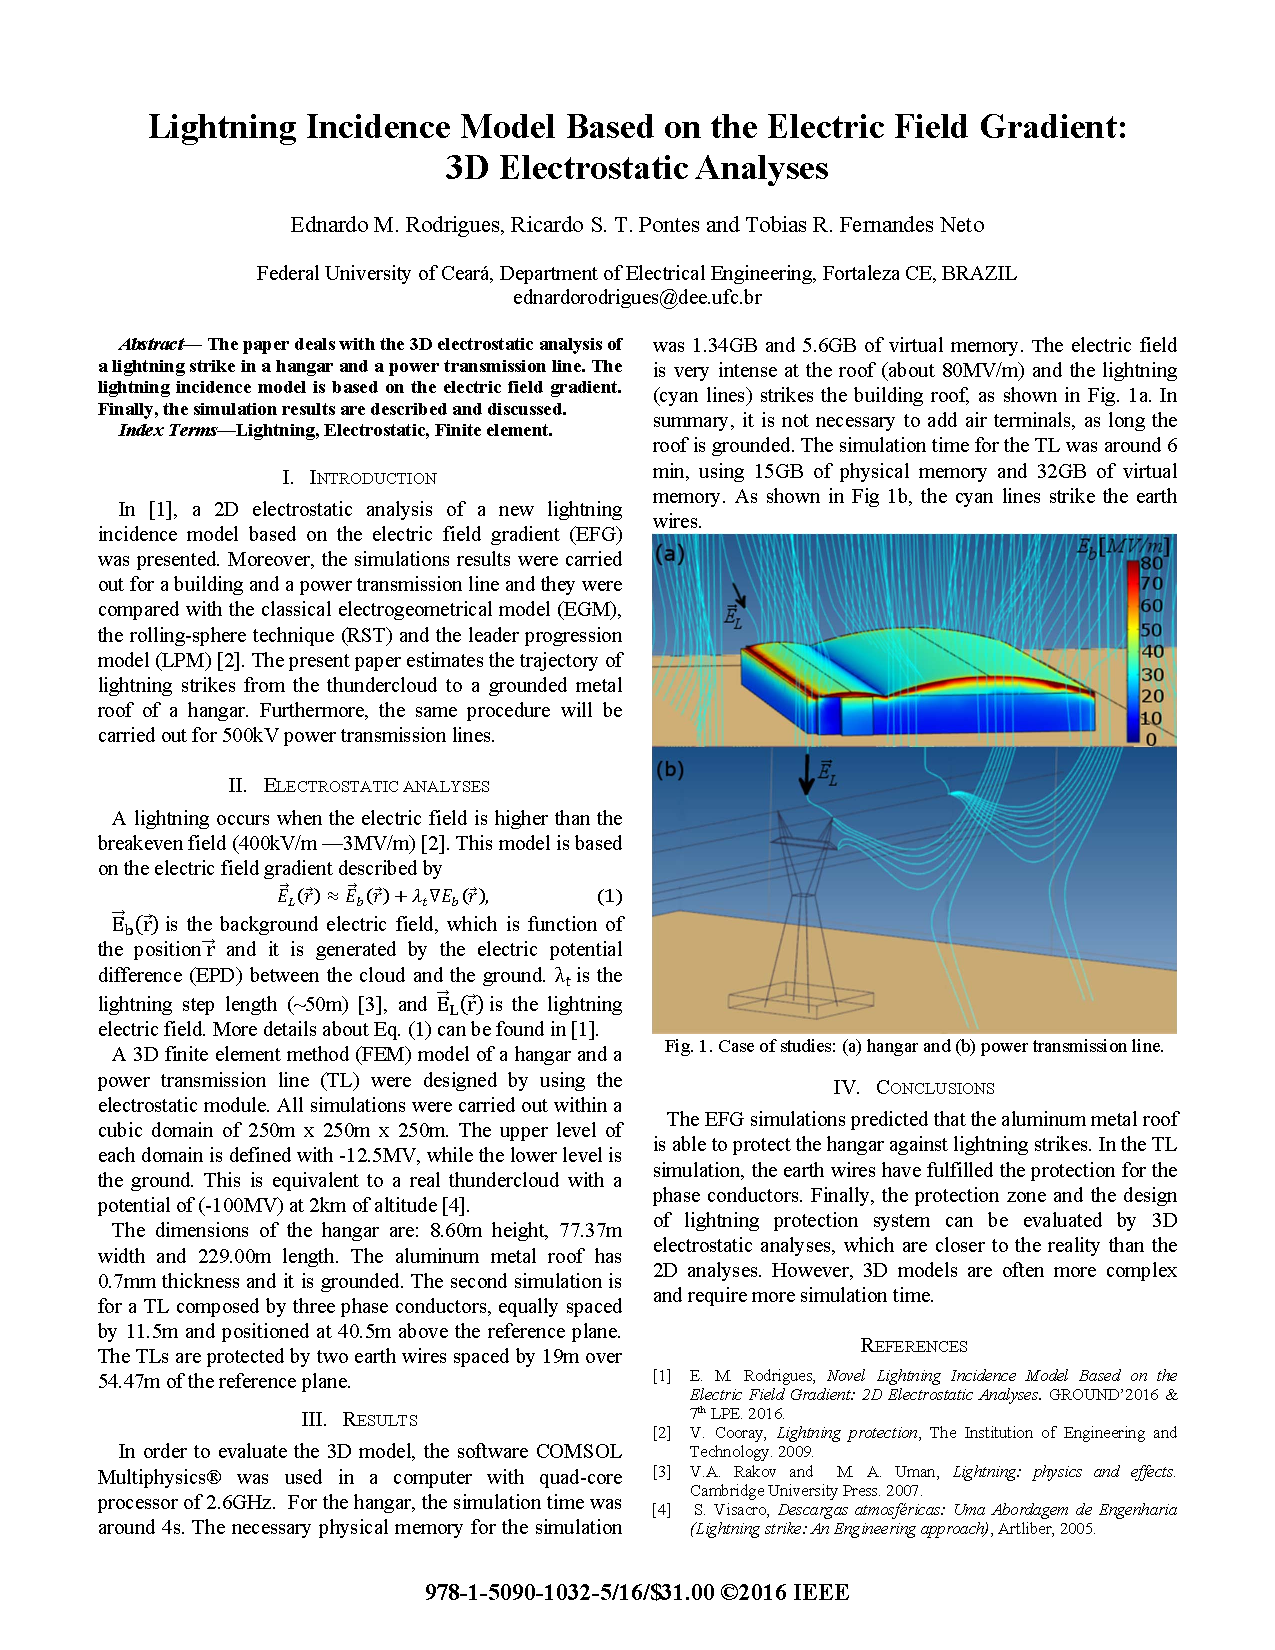
\includepdf[pages={-}]{3-pos-textuais/apendices/PID4416093.pdf}
	\imprimiranexos
		% Adicione aqui os anexos do seu trabalho
		% anexo-a/b são exemplos do template, sem relação com este TCC —
		% desativados até que o autor tenha anexos reais para incluir.
		%\anexo{Exemplo de um anexo}
\label{an:ex_anexo_a}

Um anexo é um documento que não foi elaborado pelo autor, ou seja, o autor apenas anexa. Anexos podem ser tabelas, mapas, diagramas, \textit{datasheets}, manuais e etc. 




		%\anexo{Exemplo de um anexo em PDF}
\label{an:ex_anexo_b}

O autor pode anexar um \gls{PDF}, traduzido como formato portátil de documento. Veja o código fonte utilizado para anexar o arquivo ``Sikasil.pdf'' que foi colocado dentro da pasta ``anexos'' que por sua vez está dentro da pasta ``elementos-pos-textuais''. Tenha muita atenção na hora de especificar o local do arquivo. Recomenda-se não utilizar caracteres especiais para nomear pastas e, principalmente, arquivos. 

Pode-se fazer uma descrição sucinta do arquivo anexado.

%Comando para incluir um arquivo em PDF:
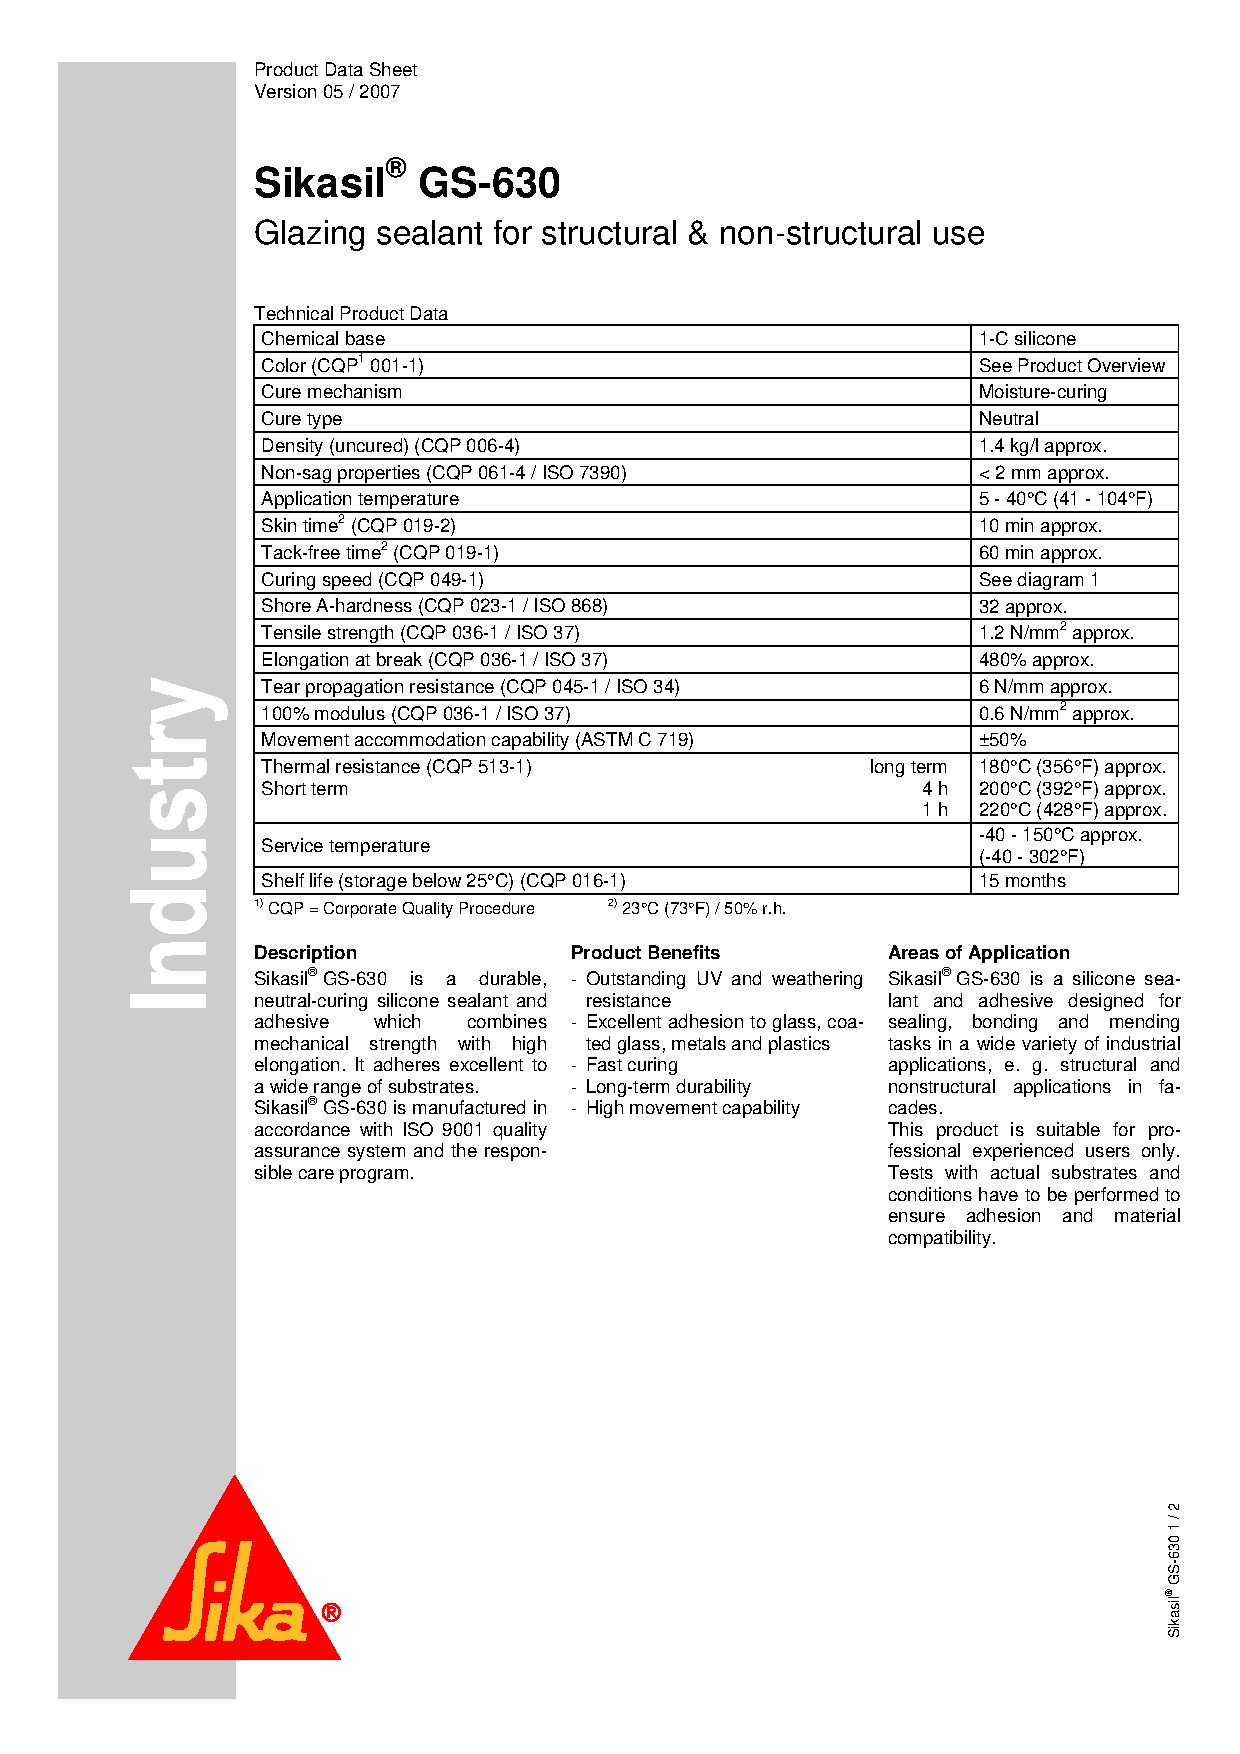
\includepdf[pages={-}]{3-pos-textuais/anexos/Sikasil.pdf}


	\imprimirindice
	\fi

\end{document}